\begin{figure}[h]
\centering
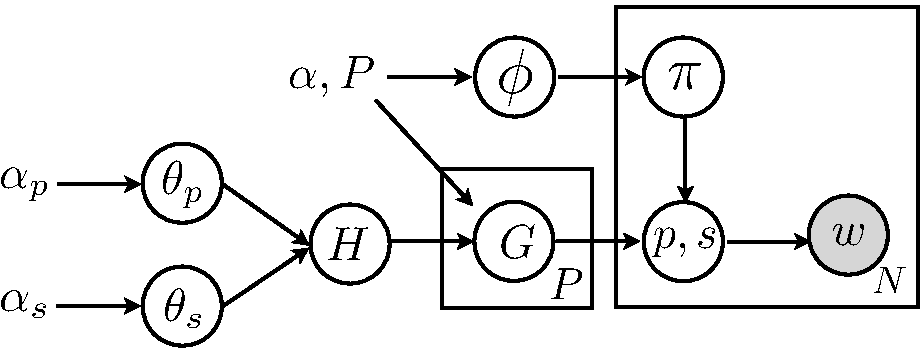
\includegraphics[width=0.4\textwidth]{fig/v3}
\caption{Parallelized model}
\label{fig:v1}
\end{figure}

\begin{align*}
\theta_p & \sim \text{Dir}(\alpha_p) \\
\theta_s & \sim \text{Dir}(\alpha_s) \\
H(p, s) & = p(p \mid \theta_p) p(s \mid \theta_s) \\
\phi & \sim \text{Dir}\left(\frac{\alpha}{P}\right) \\
\forall j \in \{1 \dots P\} \\
G_j & \sim \text{DP}\left(\frac{\alpha}{P}, H\right)\\
\forall i \in \{1 \dots N\} \\
\pi_i & \sim \phi \\
(p_i, s_i) & \sim G_{\pi_i} \\
w_i & = p_i+s_i
\end{align*}
